\documentclass[a4paper, 11pt]{report}
\usepackage[utf8]{inputenc}
\usepackage[T1]{fontenc}
\usepackage[colorlinks=true, urlcolor=purple, linkcolor=blue, pdftitle={Projet Optimisation}, pdfauthor={Adrien TALATIZI, Alexandre MARIN}, pdfsubject={optimisation}, pdfkeywords={master I.M.P.E., optimisation, MATLAB}]{hyperref}
\usepackage[french]{babel}
\usepackage{xspace}
\usepackage{textcomp}
\usepackage[table]{xcolor}

\usepackage{array}
\usepackage{amsmath}
\usepackage{amssymb}
%\usepackage{amsthm}
%\usepackage[french]{algorithm2e}
\usepackage{graphicx}
\usepackage{listings}
\usepackage{mathrsfs}

\newcounter{question}
\renewcommand\thesection{\arabic{section}}
\renewcommand\thequestion{Question 1.4.\arabic{question}}
\newcommand\question{\addtocounter{question}{1}\vspace*{1cm}{\raggedright\textbf{\thequestion}}\par\vspace*{0.5cm}}


%important quantities
\newcommand\propellantsvlct[1]{\mathrm{v}_{\mathrm{e}\,#1}}%velocity of the propellants
\newcommand\masspropel[1]{\mathrm{m}_{\mathrm{e}\,#1}}%propelling velocity
\newcommand\massstruct[1]{\mathrm{m}_{\mathrm{s}\,#1}}%mass of the structure
\newcommand\constructidx[1]{\mathrm{k}_{#1}}%constructive index
\newcommand\initmass[1]{\mathrm{M}_{\mathrm{i}\,#1}}%initial mass
\newcommand\finalmass[1]{\mathrm{M}_{\mathrm{f}\,#1}}%final mass
\newcommand\propellingvlct{\mathrm{V}_{\mathrm{p}}}%propelling velocity
\newcommand\realvlct{\mathrm{V}_{\mathrm{r}}}%real velocity
\newcommand\targetvlct{\mathrm{V}_{\mathrm{c}}}%target velocity
\newcommand\payload{\mathrm{m}_{\mathrm{u}}}%payload
\newcommand\targetalt{\mathrm{H}_{\mathrm{c}}}%target altitude


\includeonly{intro, analytical_part}


\begin{document}

\lstset{%
basicstyle=\color{black}\ttfamily,%
keywordstyle=\color{blue}\bfseries\ttfamily,%
identifierstyle=, %
commentstyle=\color{green}\slshape, %
stringstyle=\ttfamily, %
showstringspaces=true,%
language=MATLAB,%
frame=none,%
numbers=none}



\begin{titlepage}
\author{Adrien TALATIZI\\ Alexandre MARIN}
\date{pour le 7 janvier 2020}
\title{Projet Optimisation\\ Optimisation d'un lanceur spatial}
\maketitle
\tableofcontents
\end{titlepage}


\section{Introduction}

Ce projet d'optimisation, qui est un module du master \emph{Ingénierie Mathématique Pour l'Entreprise}, consiste à configurer un lanceur spatial afin de mettre sur orbite un satellite. Dans notre cas, il s'agit d'amener une masse utile $m_{\textrm{u}}=1~500~\textrm{kg}$ en orbite, à l'altitude $R_{\textrm{c}}=200~\textrm{km}$.

Dans ce rapport, nous décrivons d'abord succinctement la fonction \lstinline+SQP+, nous résumons les cas tests, nous expliquons ensuite l'optimisation du lanceur et nous présentons enfin les résultats issus de cette optimisation.

Les réponses aux questions en rapport avec la résolution analytique sont également données.

\vspace{2cm}

L'arborescence du projet s'organise comme suit, avec ces dossiers :
\vspace{1cm}
\begin{itemize}
\item\lstinline+SQP+ contient les fichiers nécessaires au fonctionnement de l'algorithme SQP ;
\item\lstinline+simulator+ contient deux fonctions permettant l'intégration numérique pour le problème de trajectoire ;
\item\lstinline+solving+ contient des scripts résolvant les problèmes posés dans le cadre de ce projet ;
\item\lstinline+tests+ rassemble des tests des fonctions contenues dans les dossiers \lstinline+SQP+ et \lstinline+simulator+.
\end{itemize}

\include{SQP}
%Adrien's part
\section{Présentation des résultats sur les deux cas tests}

\begin{center} \emph{\textbf{PREMIER CAS TEST} : polynôme}\\\end{center}

\renewcommand{\labelitemi}{\textbullet}
\begin{itemize}
\item On définit la fonction test \textit{f} t.q.\\
$f(x_1,x_2,x_3,x_4,x_5) = (x_1-1)^2+(x_1-x_2)^2 + (x_2 - x_3)^3 + (x_3 - x_4)^4 + (x_4 - x_5)^4$\\
\item Et la contrainte \textit{c} t.q.\\
$c(x_1,x_2,x_3,x_4,x_5) =
(x_1 + x_2)^2 + x_3^2 - 3\sqrt{2} - 2 , 
x_2 - x_3^2 + x_4 - 2\sqrt{2} + 2 , 
x_{1}x_{5} - 2)^{T}$;\bigbreak
\end{itemize}

\begin{itemize}
\item On prend comme point de départ de l'algorithme SQP : $x^0 = (-1 ; 2 ; 1 ; -2 ; -2)^{T}$\\
\indent avec pour objectifs : $x^{*} = (-1.2366 ; 2.4616 ; 1.1911 ; -0.2144 ; -1.6165)^{T}$ et $f(x^{*}) = 28.4974$\\
\end{itemize}
Les résultats sont stockés dans le tableau suivant : \smallbreak
{\renewcommand{\arraystretch}{1.5}\setlength{\tabcolsep}{3pt}
\begin{table}[h]\centering \small\begin{tabular}{|c|c|c|c|c|c|c|}
	\hline
 	iter & x & f(x) & $\| $c(x)$ \|$ & $\|    \nabla $L$  \|$ & rho & appels de f et c\\
	\hline
 	0 & $( -1, 2, 1, -2, -2 )^{T}$ & 95.0 & 2.8935 & 62.7595 & / & 6\\
	\hline
 	1 & $(-0.937, 2.16, 1.49, 0.0856, -1.9165)^{T}$ & 33.62 & 0.877 & 194.896 & 52.196759 & 12\\
	\hline
 	2 & $( -1.54, 2.2954, 1.49, 0.09, -1.32 )^{T}$ & 29.4057 & 0.73 & 42.71 & 12.824709 & 20\\
	\hline
 	3 & $( -0.9, 2.49, 1.07, -0.51, -1.85 )^{T}$ & 27.871 & 0.32 & 6.514 & 10.790444 & 26\\
	\hline
 	4 & $( -1.21, 2.45, 1.21, -0.17, -1.592 )^{T}$ & 27.94 & 0.078 & 2.52 & 10.112978 & 32\\
	\hline
 	5 & $( -1.2595, 2.4669, 1.19, -0.22, -1.588 )^{T}$ & 28.53 & 98e-5 & 1.454 & 10.005331 & 38\\
	\hline
 	6 & $( -1.2393, 2.4623, 1.19, -0.22, -1.61)^{T}$ & 28.504 & 518e-6 & 0.237 & 9.942327 & 44\\
	\hline
 	7 & $( -1.237, 2.46, 1.19, -0.216, -1.6169 )^{T}$ & 28.50865 & 8.178e-06 & 9.963e-3 & 9.897096 & 50\\
	\hline
 	8 & $( -1.237, 2.46, 1.19, -0.21565, -1.6168 )^{T}$ & 28.508725 & 2.61e-09 & 48e-6 & 9.896991 & 56\\
	\hline
 	9 & $( -1.237, 2.462, 1.19, -0.21565, -1.6168 )^{T}$ & 28.5087 & 2.077e-12 & 3.1395e-07 & 9.896981 & 62\\

	\hline
\end{tabular}\end{table}
}\normalsize
\bigbreak
\textit{Note : les résultats obtenus sont bien conformes aux résultats attendus. On remarquera que sans les bornes, SQP converge vers d'autres minima locaux. Il est donc important de choisir ces bornes proches de la solution attendue. On choisit donc un intervalle de 0.6
autour de celle-ci.}
\newpage





\begin{center}\emph{\textbf{SECOND CAS TEST} : masses d'ergols de la fusée Ariane 1}\\\end{center}





\begin{itemize}
\item On définit la fonction test \textit{f} t.q.\\
$f(x_1,x_2,x_3) = 1700+1.1101x_1 + 1.1532x_2 + 1.2154x_3$\\
\item Et la contrainte \textit{c} t.q.\\
$c(x_1,x_2,x_3) =$\\
\smallbreak
$4344.3ln(\frac{1700+1.2154x_3}{1700+0.2154x_3}) 
+ 2922.4ln(\frac{1700+1.2154x_3+1.1532x_2}{1700+0.2154x_3+0.1532x_2}) 
+ 2647.2ln(\frac{1700+1.2154x_3+1.1532x_2+1.1101x_1}{1700+0.2154x_3+0.1532x_2+0.1101x_1}) 
-11527$

\bigbreak

\item On prend comme point de départ de l'algorithme SQP : $x^0 = (115000, 35000, 6000)^{T}$ qui est la moyenne des bornes\\
\indent avec pour objectifs : $x^{*} = (145349 ; 31215 ; 7933)^{T}$ et $f(x^{*}) = 208691$\\
\end{itemize}
Les résultats sont stockés dans le tableau suivant : \smallbreak
{\renewcommand{\arraystretch}{1.5}
\begin{table}[h]\centering \small\begin{tabular}{|c|c|c|c|c|c|c|}
	\hline
 	iter & x & f(x) & $\| $c(x)$ \|$ & $\|    \nabla $L$  \|$ & rho & appels de f et c\\
	\hline
	0 & $(115000, 35000, 6000)^{T}$ & 177015.90 & 361.36 & 361.36 & / & 4\\
	\hline
	1 & $(115970.49, 35416.328, 10000)^{T}$ & 183434.95 & 273.45 & 1564.81 & 81642.55 & 8\\
	\hline
	2 & $(127626.0, 44731.2, 5870.50)^{T}$ & 202096.70 & 199.55 & 87809.94 & 1001129.48 & 12\\
	\hline
	3 & $(137284.567, 50000, 6870.88 )^{T}$ & 220110.46 & 21.18 & 7113.2 & 119425.29 & 16\\
	\hline
	4 & $(138609.19, 50000, 6991.44 )^{T}$ & 221727.45 & 1.35& 185.21 & 3332.76 & 20\\
	\hline
	5 & $(138700.45, 49991.19216, 6999.994 )^{T}$ & 221829.01 & 13e-4 & 3.84 & 90.44 & 24\\
	\hline
	6 & $(138700.47, 49971.01733, 7000.62 )^{T}$ & 221806.52 & 6.4e-05 & 3.13 & 76.58 & 28\\
	\hline
	7 & $(138539.77, 20000, 8529.26 )^{T}$ & 188923.47 & 235.69 &235.71 & 128.95 & 32\\
	\hline
	8 & $(137507.1, 30996.5, 7875.68)^{T}$ & 199663.91 &  79.98 & 79.98 & 100.46 & 36\\
	\hline
	9 & $(143378.6, 32532.79, 8406.05 )^{T}$ & 208598.11 & 3.37 & 3.44 & 126.30 & 40\\
	\hline
	10 & $(143403.19, 32874.4, 8379.81 )^{T}$ & 208987.45 & 0.045 & 0.61 & 122.72 & 44\\
	\hline
\end{tabular}
\end{table}}
\bigbreak
\textit{Note : les résultats obtenus sont bien conformes au résultats attendus. On remarquera que sans les bornes, SQP converge vers d'autres minima locaux. Il est donc important de choisir ces bornes proches de la solution attendue. On choisit donc de poser la borne supérieure comme étant $(170000 , 50000 , 10000)^{T}$ et la borne inférieure comme $(60000 , 20000 , 2000)^{T}$. Cela nous évite de plus de converger vers des solutions non physiques.}


\include{launcher_optim}
\section{Résolution analytique du problème d'étagement}

On reprend les notations de l'énoncé, indications comprises.

\question Notons que pour $j\in\{1,2,3\}$,
\begin{align*}
\dfrac{\initmass{j+1}}{\initmass{j}} &= \dfrac{\finalmass{j}-\massstruct{j}}{\initmass{j}} =%
\dfrac{\finalmass{j}-\constructidx{j}\masspropel{j}}{\initmass{j}} \\ &= \dfrac{\finalmass{j}-\constructidx{j}(\initmass{j}-\finalmass{j})}{\initmass{j}} = \dfrac{1+\constructidx{j}}{x_{j}}-\constructidx{j}\text{.}
\end{align*}

Notons $\varphi$ l'application qui envoie $(\masspropel{1},\masspropel{2},\masspropel{3})$ sur $x$ par la formule
\[x_{j} = 1 + \dfrac{\masspropel{j}}{\payload + \sum_{j<l\leqslant 3}(1+\constructidx{l})\masspropel{l} \,+ \constructidx{j}\masspropel{j}}\text{.}\]
Alors $\varphi$ est bijective car pour tout $j\in\{1,2,3\}$
\[\masspropel{j}=\dfrac{\payload + \sum_{j<l\leqslant 3}(1+\constructidx{l})\masspropel{l}}{1+\constructidx{j}(1-x_{j})}\]
et donc $J=-f\circ \varphi$. La reformulation de la contrainte étant immédiate, les deux problèmes considérés sont équivalents.

\question Si $x$ est un minimiseur local de $f$ sous la contrainte $c$, comme ces deux fonctions sont de classe $\mathscr{C}^1$ et que la contrainte en $x$ est forcément qualifiée, il existe $\lambda\in\mathbb{R}$ tel que, pour tout $j\in\{1,2,3\}$
\[\dfrac{\partial f}{\partial x_{j}}(x) + \lambda\dfrac{\partial c}{\partial x_{j}}(x) = 0\]
avec
\[\dfrac{\partial f}{\partial x_{j}}(x) = y_{j+1}\,y_{j+2}\left(\dfrac{1+\constructidx{j}}{x_{j}^{2}}\right)%
,\; \dfrac{\partial c}{\partial x_{j}}(x) = \dfrac{\propellantsvlct{j}}{x_{j}}\]
en considérant des indices \emph{modulo} $3$.

En multipliant l'équation ci-desssus par $x_j$ et en remarquant que
\[f(x)=-y_{1}\,y_{2}\,y_{3},\; 1+\dfrac{\constructidx{j}}{y_{j}}=(1-\Omega_{j}x_{j})^{-1}\]
on obtient
\[\propellantsvlct{j}(1-\Omega_{j}x_{j}) = \dfrac{f(x)}{\lambda}\text{.}\]

\question Dans l'équation qui précède, le membre de droite ne dépend pas de $j$, donc
\[x_{j} = \dfrac{1}{\Omega_{j}}\left[1-\dfrac{\propellantsvlct{3}}{\propellantsvlct{j}}(1-\Omega_{3}x_{3})\right]\]
et on voit que le problème revient à résoudre $c(x)=0$ où $x_1$ et $x_2$ s'expriment en fonction de $x_3$.

\question On considère une vitesse propulsive $\propellingvlct = 1.2\,\targetvlct$. Dans le fichier \verb+analytical_approach.m+ du dossier \verb+solving+, nous résolvons cette équation en $x_3$ avec la méthode de Newton. On obtient

\begin{center}
$\begin{array}{|c|c|c|c|c|c|}\hline
x_3 & \masspropel{1} & \masspropel{2} & \masspropel{3} & \mathrm{M}_{0} & \lambda\\\hline
3,118\,9 & 26\ 981\text{ kg}& 12\ 704\text{ kg} & 5\ 516\text{ kg} & 52\ 408\text{ kg} & -1,354\,7\cdot 10^{-5}\\\hline
\end{array}$
\end{center}

La troisième équation donnée par le théorème de K.K.T. nous conduit au nombre $-3,47\cdot 10^{-18}$.


\section{Résultats}

\subsection{Résultats numériques}

Les grandeurs physiques ont pour unités celles du système international.

Les itérations sur la vitesse propulsive sont effectuées dans le script \lstinline+set_config.m+~: les problèmes d'étagement et de trajectoire sont résolus respectivement grâce aux fichiers \lstinline+stage_solver.m+ et \lstinline+path_solver.m+.

Voici les résultats issus de l'exécution de \lstinline+set_config.m+~:

\[\begin{array}{|c|c|c|c|c|c|}\hline
\text{itération} & \masspropel{} & \propellingvlct & \realvlct & \mathrm{M}_0 & \theta\\ \hline
1 & \begin{pmatrix}27\,144\\ 12\,564\\ 5\,501\end{pmatrix} & 9\,341 & 7\ 801 & 52\,408 & %
\begin{pmatrix}0,053\\ -0,013\,768\\ 0,326\,8\\ 0,138\,06\end{pmatrix}\\\hline
2 & \begin{pmatrix}26\,841\\ 12\,496\\ 5\,491\end{pmatrix} & 9\,324 & 7\ 781 & 51\,984 & %
\begin{pmatrix}0,053\\ -0,013\,727\\ 0,327\,56\\ 0,139\,06\end{pmatrix}\\\hline
\end{array}\]

La vitesse cible $\targetvlct$ vaut dans notre cas $7\,784,26$.

\subsection{Graphes : trajectoire, altitude, vitesse et masse}

Les graphes présentés ici correspondent à la configuration optimale du lanceur.

Voici les durées de combustion et instants $t_j$ de fin de combustion pour chaque étage~:

\[\begin{array}{|c|c|c|}\hline
\durcombustion{1} & \durcombustion{2} & \durcombustion{3}\\\hline
89,5 & 166,9 & 298,7\\\hline
\end{array}\]

\[\begin{array}{|c|c|c|}\hline
t_{1} & t_{2} & t_{3}\\\hline
\durcombustion{1} & 256,4 & 555,1\\\hline
\end{array}\]

\clearpage
\begin{center}
\begin{figure}[htbp]
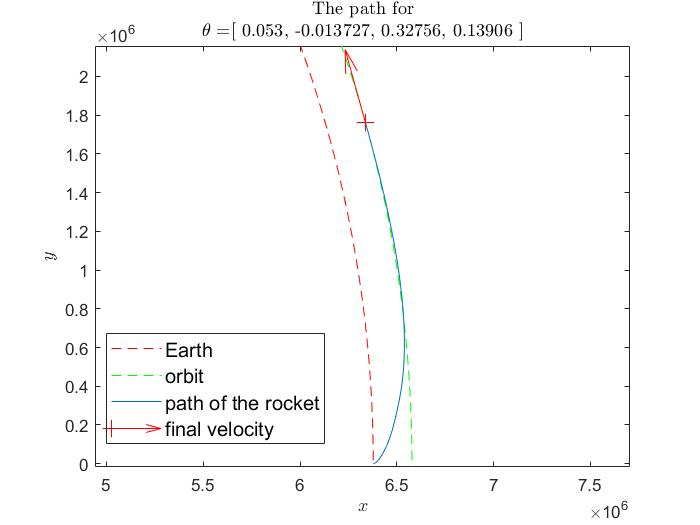
\includegraphics[scale=0.65]{./graphs/path.jpg}
\caption{trajectoire de la fusée et vecteur vitesse final}
\end{figure}
\end{center}

D'après ce graphe, il semble que l'altitude cible est atteinte et que le vecteur vitesse final est bien tangent à l'orbite visée.

\clearpage
\begin{center}
\begin{figure}[t]
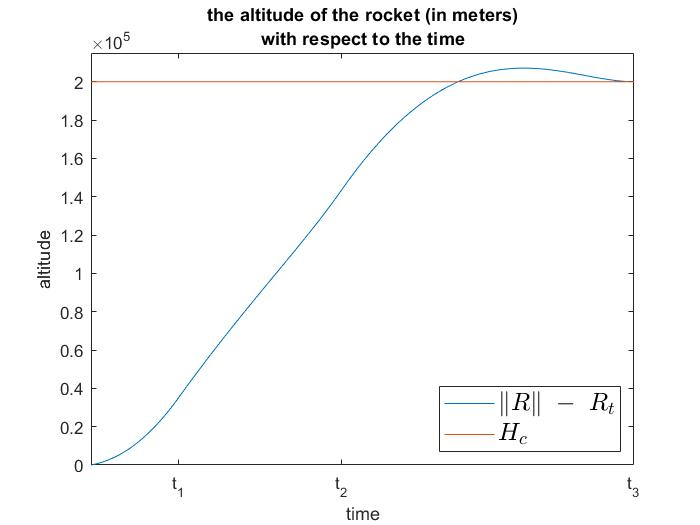
\includegraphics[scale=0.65]{./graphs/altitude.jpg}
\caption{altitude de la fusée en fonction du temps}
\end{figure}
\end{center}

L'altitude cible est bien atteinte selon ce graphe.

\clearpage
\begin{center}
\begin{figure}[t]
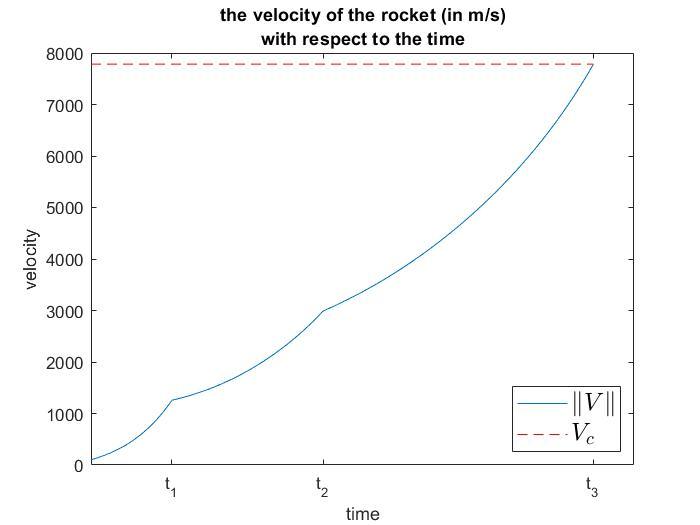
\includegraphics[scale=0.65]{./graphs/velocity.jpg}
\caption{vitesse de la fusée en fonction du temps}
\end{figure}
\end{center}

On peut s'assurer avec ce graphe que la vitesse cible est vraiment atteinte.

\clearpage
\begin{center}
\begin{figure}[t]
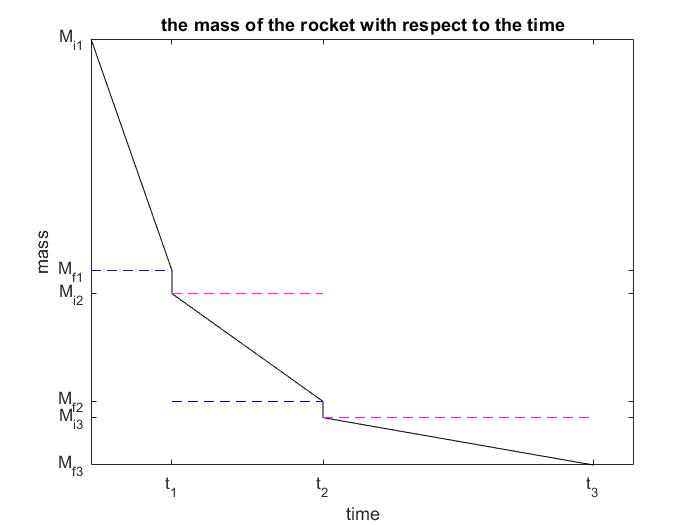
\includegraphics[scale=0.65]{./graphs/mass.jpg}
\caption{masse de la fusée en fonction du temps}
\end{figure}
\end{center}

La masse est bien une fonction affine par morceaux. La masse utile n'a pas été représentée afin de rendre le graphe plus clair.


\end{document}